% =====================================================================
%  Learning Quantum Dynamics via Fourier Coefficient Extraction
%  M2 QMI Internship Project -- Thomas Lagoutte
%  Supervisor: Prof. Koji Terashi (ICEPP, U.~Tokyo)
%
%  Build:
%     latexmk -pdf -shell-escape main.tex
%     (or: pdflatex main && pdflatex main)
%
%  Required packages (most TeX Live full installs ship these):
%     beamer, beamertheme-metropolis (mtheme), tikz, quantikz,
%     pgfplots, physics, mathtools, booktabs, listings, hyperref.
% =====================================================================
\documentclass[aspectratio=169,11pt,xcolor={dvipsnames,table}]{beamer}

% =====================================================================
%  THEME & TYPOGRAPHY
% =====================================================================
\usetheme[progressbar=frametitle, numbering=fraction, block=fill]{metropolis}
\usepackage[T1]{fontenc}
\usepackage{lmodern}
\usepackage[english]{babel}
\usepackage{microtype}

% Sober academic palette (IPP navy + ICEPP/U-Tokyo accents)
\definecolor{IPPblue}{RGB}{0,51,102}
\definecolor{IPPaccent}{RGB}{197,36,50}
\definecolor{TokyoBlue}{RGB}{0,80,152}
\definecolor{SoftGray}{RGB}{240,240,240}

\setbeamercolor{normal text}{fg=black, bg=white}
\setbeamercolor{alerted text}{fg=IPPaccent}
\setbeamercolor{progress bar}{fg=IPPblue}
\setbeamercolor{title separator}{fg=IPPblue}
\setbeamercolor{frametitle}{bg=IPPblue, fg=white}
\setbeamercolor{block title}{bg=IPPblue!10, fg=IPPblue}
\setbeamercolor{block body}{bg=IPPblue!3, fg=black}

% =====================================================================
%  MATH / PHYSICS / GRAPHICS
% =====================================================================
\usepackage{amsmath,amssymb,amsthm,amsfonts,mathtools,bm}
\usepackage{braket}     % \ket, \bra, \braket
\usepackage{xspace}

% Lightweight stand-ins for the `physics` package macros we use
\providecommand{\expval}[1]{\left\langle #1 \right\rangle}
\providecommand{\ketbra}[2]{\ket{#1}\!\bra{#2}}
\providecommand{\dyad}[1]{\ket{#1}\!\bra{#1}}
\providecommand{\Tr}{\operatorname{Tr}}
\providecommand{\identity}{\mathbb{1}}
\usepackage{graphicx}
\graphicspath{{../}{./figures/}{./}}
\usepackage{tikz}
\usetikzlibrary{arrows.meta,calc,positioning,fit,backgrounds,decorations.pathreplacing}
\usepackage{quantikz}
\usepackage{booktabs,multirow,array}
\usepackage{caption}
\captionsetup[figure]{font=footnotesize, labelfont=bf}

% Code listings (Python, used in implementation slides)
\usepackage{listings}
\lstdefinestyle{py}{%
  basicstyle=\ttfamily\scriptsize,
  language=Python,
  keywordstyle=\color{IPPblue}\bfseries,
  commentstyle=\color{gray}\itshape,
  stringstyle=\color{IPPaccent},
  showstringspaces=false, breaklines=true,
  frame=single, rulecolor=\color{SoftGray}, framerule=0.3pt,
  xleftmargin=4pt, xrightmargin=4pt
}

\usepackage{hyperref}
\hypersetup{colorlinks=true, urlcolor=IPPblue, linkcolor=IPPblue, citecolor=IPPblue}

% =====================================================================
%  CUSTOM MACROS  (used throughout the talk)
% =====================================================================
\newcommand{\BQP}{\mathsf{BQP}}
\newcommand{\Ppoly}{\mathsf{P/poly}}
\newcommand{\BPP}{\mathsf{BPP}}
\newcommand{\PQC}{\textsc{PQC}\xspace}
\newcommand{\PAC}{\textsc{PAC}\xspace}
\newcommand{\Algo}{\mathcal{A}}
\newcommand{\Hyp}{\mathcal{H}}
\newcommand{\Cclass}{\mathcal{C}}
\newcommand{\Dist}{\mathcal{D}}
\newcommand{\Real}{\mathbb{R}}
\newcommand{\Integers}{\mathbb{Z}}
\newcommand{\Complex}{\mathbb{C}}
\newcommand{\Lspace}{\mathcal{L}}
\newcommand{\Sphere}{\mathbb{S}}
\renewcommand{\vec}[1]{\bm{#1}}
\newcommand{\xvec}{\vec x}
\newcommand{\avec}{\vec\alpha}
\newcommand{\wvec}{\vec w}
\newcommand{\bvec}{\vec b}
\newcommand{\norm}[1]{\left\lVert#1\right\rVert}
\newcommand{\fhat}{\hat f}

% Theorem / definition environments
\newtheorem{thmA}{Theorem}
\newtheorem{lemA}[thmA]{Lemma}
\newtheorem{corA}[thmA]{Corollary}
\theoremstyle{definition}
\newtheorem{defA}[thmA]{Definition}

% Speaker notes (uncomment to project notes on second screen)
% \setbeameroption{show notes on second screen=right}

% =====================================================================
%  TITLE METADATA
% =====================================================================
\title{Learning Quantum Dynamics via\\Fourier Coefficient Extraction}
\subtitle{Theory, algorithms and implementation}
\author{Thomas Lagoutte}
\institute{M2 QMI -- Institut Polytechnique de Paris\\ICEPP, The University of Tokyo}
\date{\today}

% =====================================================================
\begin{document}
% =====================================================================

% ---------------------------------------------------------------------
%  SLIDE 01 -- Title page
% ---------------------------------------------------------------------
{%
\setbeamertemplate{footline}{}            % hide footline on title slide
\begin{frame}[plain,noframenumbering]

  \vspace*{-0.55cm}

  % --- Title block -------------------------------------------------
  \begin{center}
    {\color{IPPblue}\rule{\linewidth}{0.6pt}}\\[0.4em]
    {\large\bfseries Learning Quantum Dynamics via\\[0.05em]
                     Fourier Coefficient Extraction}\\[0.25em]
    {\small\itshape Theory, algorithms and implementation}\\[0.30em]
    {\color{IPPblue}\rule{\linewidth}{0.6pt}}\\[0.30em]
    {\scriptsize After A.~Barthe, M.~Yaghubi Rad, M.~Grossi \& V.~Dunjko,\;
     \href{https://arxiv.org/abs/2506.17089}{\texttt{arXiv:2506.17089}} (2025)}
  \end{center}

  \vspace{0.35em}

  % --- Author + affiliations --------------------------------------
  \begin{center}
    {\normalsize\bfseries Thomas Lagoutte}\\[0.15em]
    {\scriptsize M2 \emph{Quantum Devices, Materials and Information} (QMI)\,---\,Institut Polytechnique de Paris}\\[0.05em]
    {\scriptsize Internship at ICEPP, The University of Tokyo}\\[0.20em]
    {\footnotesize Supervisor: \textbf{Prof.~Koji Terashi}}\\[0.15em]
    {\scriptsize \today}
  \end{center}

  \vspace{0.30em}

  % --- Roadmap teaser ---------------------------------------------
  \begin{center}
    \begin{minipage}{0.96\linewidth}\centering
      \scriptsize\color{IPPblue}
      \textbf{Roadmap.}\;
      \textbf{I.}~Theory \& proofs (PAC, Algorithm \(A\), classical hardness)
      \;$\bullet$\;
      \textbf{II.}~Implementation stack (Qiskit, registers, pipeline)
      \;$\bullet$\;
      \textbf{III.}~Numerical results (TFIM, Schwinger, shot-noise)
    \end{minipage}
  \end{center}

  \vfill

  % --- Logo strip (in-flow, no TikZ overlay to avoid overlap) ------
  \noindent
  \begin{minipage}[c]{0.32\linewidth}\centering
    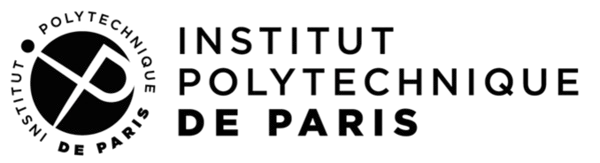
\includegraphics[height=0.75cm]{ipp_logo.png}
  \end{minipage}\hfill
  \begin{minipage}[c]{0.32\linewidth}\centering
    
\includegraphics[height=0.75cm]{utokyo_logo.png}
  \end{minipage}\hfill
  \begin{minipage}[c]{0.32\linewidth}\centering
    
\includegraphics[height=0.75cm]{icepp_logo.png}
  \end{minipage}

  \vspace*{-0.05cm}

  % --- Speaker notes (use \setbeameroption{show notes...} to display)
  \note{%
    Open with one short sentence: ``Today I will reconstruct the proof
    that learning Hamiltonian dynamics admits a provable BQP-vs-classical
    separation under the PAC framework, and I will show how I implemented
    the underlying algorithm.'' \\
    Mention: paper is from June 2025, joint Leiden + CERN. \\
    Frame the talk as three acts: theory, code, results -- ask audience
    to hold questions for end of each part.
  }
\end{frame}
}

% ---------------------------------------------------------------------
%  PART I -- THEORY
% ---------------------------------------------------------------------

% =====================================================================
%  SLIDE 02 -- Motivation: The Learning Problem
% =====================================================================
\begin{frame}{Motivation\,---\,Learning Quantum Dynamics from Classical Data}

  \scriptsize
  \textbf{Supervised task.}~Given i.i.d.\ samples
  \(\mathcal D_T=\{(\xvec_t,y_t)\}_{t=1}^{T}\sim\Dist^{T}\) with labels
  \(y_t = f_{\avec}(\xvec_t)\), where
  \[
    f_{\avec}(\xvec)\;=\;\bra{\psi(\xvec,\avec)}\,O\,\ket{\psi(\xvec,\avec)},
    \qquad
    \ket{\psi(\xvec,\avec)}=e^{\,i\,H(\xvec,\avec)\,t}\ket{\psi_0},
  \]
  return \(h\) that \(\varepsilon\)\nobreakdash-approximates \(f_{\avec}\) on
  unseen \(\xvec\sim\Dist\) (PAC sense, formalised next slide).

  \vspace{-0.2em}
  \begin{columns}[T,onlytextwidth]
    % ---- left column: physics + algorithmic content --------------
    \begin{column}{0.50\textwidth}
      \scriptsize
      \textbf{Two faces of the same concept class}\\[-0.2em]
      \begin{itemize}\setlength\itemsep{1pt}
        \item \alert{Hamiltonian dynamics} (physical):
              \(\,f_{\avec}(\xvec)=\bra{\psi(\xvec,\avec)}O\ket{\psi(\xvec,\avec)}\).
        \item \alert{PQC functions} (algorithmic):
              \(\,h_{\avec}(\xvec)=\bra{0}U^{\dagger}(\xvec,\avec)\,O\,U(\xvec,\avec)\ket{0}\).
        \item Bridged by Hamiltonian simulation (Trotter, qubitization, LCU).
      \end{itemize}

      \smallskip
      \textbf{Knowns vs.\ unknowns}\\[-0.2em]
      \begin{itemize}\setlength\itemsep{1pt}
        \item \(\xvec\): per-sample data (e.g.\ lattice mask \(x_{ij}\!\in\!\{0,1\}\)).
        \item \(\avec\!\in\![0,1]^{d}\): \emph{unknown, fixed} global couplings
              (transverse field, mass, gauge coupling, \ldots).
      \end{itemize}
    \end{column}
    % ---- right column: figure ------------------------------------
    \begin{column}{0.49\textwidth}
      \centering
      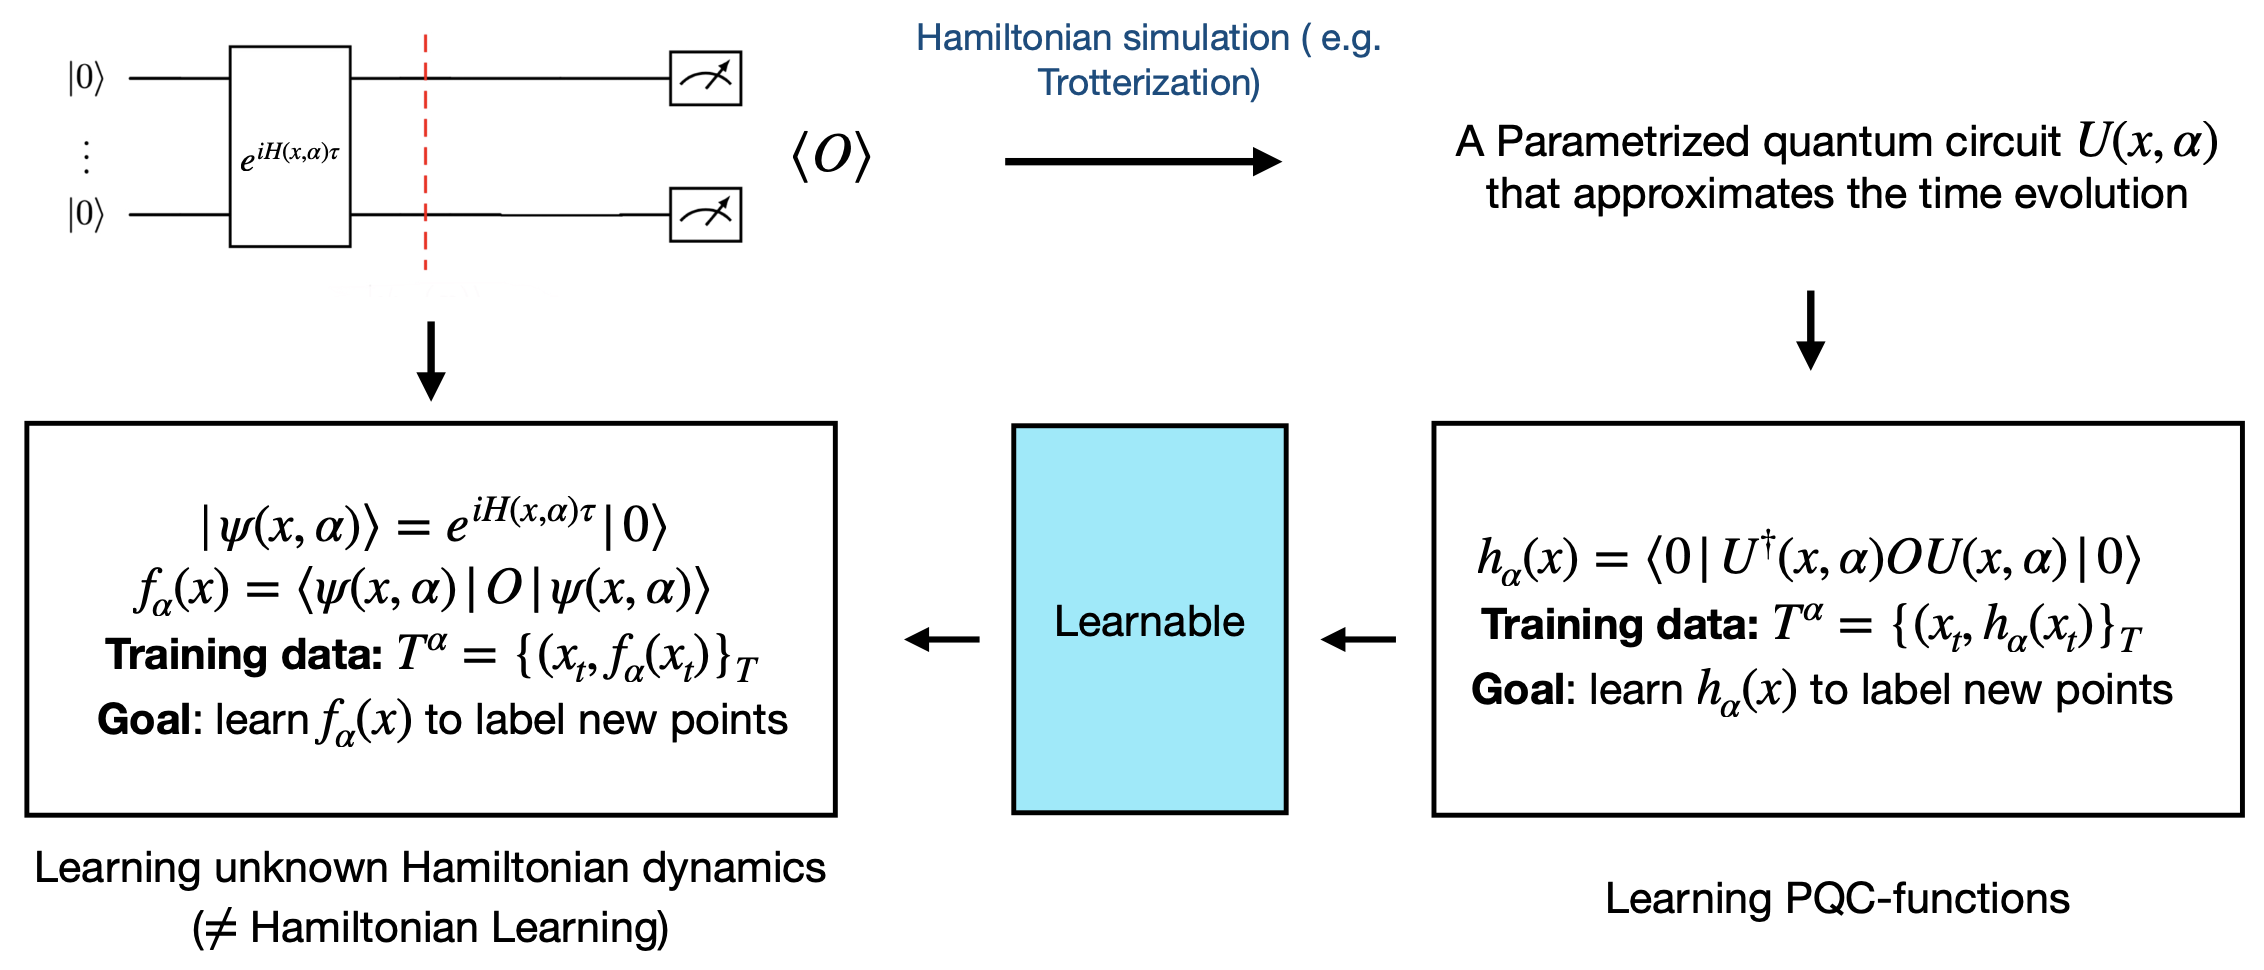
\includegraphics[width=0.95\linewidth]{pac_learning_workflow.png}\\[-0.1em]
      {\tiny\itshape Bridge between physical dynamics and PQC
       functions; PAC-learnability transfers across it.
       \emph{Adapted from} Barthe \emph{et al.}\ (2025).}
    \end{column}
  \end{columns}

  \vspace{-0.2em}
  \begin{alertblock}{\small Central question}
    \scriptsize
    Evaluating \(f_{\avec}(\xvec)\) is generically
    \(\BQP\)\nobreakdash-hard \(\Rightarrow\)
    a classical learner cannot even generate its own labels.
    \emph{Can quantum access to the dynamics yield a provably efficient
    PAC learner where no classical algorithm can?}
  \end{alertblock}

  \note{%
    Stress that this is \emph{not} Hamiltonian learning -- the algorithm
    is never asked to recover \(\avec\), only to predict labels of the
    induced function. \(\xvec\) is the per-instance data (e.g.\ a 0/1 mask
    of which lattice edges are active); \(\avec\) is the fixed-but-unknown
    coupling vector. The bridge in the figure is what makes the PAC
    reduction possible: prove the result on PQCs, then transfer to physical
    Hamiltonians via Trotterization.
  }
\end{frame}

% =====================================================================
%  SLIDE 03a -- PAC Learning: the formal definition
% =====================================================================
\begin{frame}{Probably Approximately Correct (PAC) Learning\,---\,definition}

  \footnotesize
  Originally introduced by L.~Valiant (1984); we use the
  \emph{efficient, distribution-independent} formulation of
  Barthe \emph{et al.}\ (Def.\ 1).

  \begin{block}{\small Definition 1 -- Efficient PAC learnability (Barthe \emph{et al.}, 2025)}
    \scriptsize
    A concept class \(\Cclass=\{\Cclass_n\}_n\) with
    \(c:\mathcal X_n\to\mathcal Y_n\in\Cclass_n\) is
    \emph{efficiently PAC-learnable} iff there exists an algorithm
    \(\Algo\) such that, \\[-0.6em]
    \begin{center}\itshape
      \(\;\forall\,n,\;\forall\,\varepsilon{>}0,\;\forall\,\delta{\in}(0,1],\;
        \forall\,c\in\Cclass_n,\;\forall\) target distribution \(\Dist\) on \(\mathcal X_n\),
    \end{center}
    \vspace{-0.5em}
    given an i.i.d.\ training dataset
    \(\{(\xvec_t,c(\xvec_t))\}_{t=1}^{T}\sim\Dist^{T}\) of size
    \(T\in\mathrm{poly}(n,\varepsilon^{-1},\delta^{-1})\),
    \(\Algo\) returns a hypothesis
    \(h=\Algo(T,\varepsilon,\delta)\) in time
    \(\mathrm{poly}(n,\varepsilon^{-1},\delta^{-1})\) satisfying
    \[
        \Pr_{\xvec\sim\Dist}\!\bigl[\,
          \lvert h(\xvec)-c(\xvec)\rvert\le\varepsilon
        \,\bigr]\;\ge\;1-\delta.
    \]
  \end{block}

  \vspace{-0.1em}
  \footnotesize
  \textbf{Reading guide.}
  \emph{Approximately} = error \(\le\varepsilon\); \emph{Probably} = with
  confidence \(\ge 1-\delta\); \emph{Efficient} = sample size \emph{and}
  runtime polynomial in \((n,\varepsilon^{-1},\delta^{-1})\);
  \emph{Distribution-independent} = the bound must hold for \emph{any}
  \(\Dist\). \\[0.15em]
  \(\;\;\Longrightarrow\;\) a much stronger requirement than typical
  statistical-learning average-case guarantees.

  \note{%
    Walk through the quantifiers slowly: ``for every problem size, every
    accuracy, every confidence level, every target concept in the class,
    and every input distribution.'' Emphasise that ``efficient'' here is
    a triple constraint (sample, training time, hypothesis-evaluation
    time -- the hypothesis itself must run in polynomial time on a fresh
    \(\xvec\)). Distribution independence is what rules out the classical
    workaround ``just train on toy distributions''.
  }
\end{frame}

% =====================================================================
%  SLIDE 03b -- PAC Learning: quantum vs classical, separation target
% =====================================================================
\begin{frame}{PAC Learning\,---\,quantum vs.\ classical, separation target}

  \footnotesize
  PAC learnability is parameterized by the \emph{model of computation}
  granted to the learner; everything else (samples, distribution,
  guarantees) is identical.

  \begin{columns}[T,onlytextwidth]
    \begin{column}{0.50\textwidth}
      \begin{block}{\small Classical-efficient PAC}
        \scriptsize
        \(\Algo\) and \(h\) are uniform classical poly-time TMs
        (or non-uniform: belong to \(\Ppoly\)).\\[0.2em]
        Lower bounds typically come from \emph{cryptographic} or
        \emph{complexity-theoretic} hardness.
      \end{block}
    \end{column}
    \begin{column}{0.50\textwidth}
      \begin{block}{\small Quantum-efficient PAC}
        \scriptsize
        \(\Algo\) is a uniform quantum poly-time circuit; the hypothesis
        \(h\) may be evaluated by a quantum sub-routine on a fresh
        \(\xvec\).\\[0.2em]
        Same PAC bound; the only relaxation is the hardware.
      \end{block}
    \end{column}
  \end{columns}

  \vspace{0.1em}
  \footnotesize
  \textbf{The labels are quantum either way.}~~Both learners receive the
  same dataset \(\{(\xvec_t,c(\xvec_t))\}_t\); generating \(c(\xvec_t)\)
  for the concept classes we will consider already requires
  \(\BQP\) power.

  \begin{alertblock}{\small Target separation (Barthe \emph{et al.}, Thm.~2 \& Thm.~3)}
    \scriptsize
    Exhibit a family \(\Cclass\) that is
    \alert{efficiently \emph{quantum} PAC-learnable} \emph{and},
    under the standard complexity hypothesis
    \(\boxed{\BQP\not\subseteq\Ppoly}\),
    \alert{\emph{not} efficiently classically PAC-learnable}.
    \\[0.2em]
    \(\;\Rightarrow\;\) provable, super-polynomial quantum-classical
    learning advantage on a \emph{natural, physically motivated} task.
  \end{alertblock}

  \note{%
    Stress that the learner's \emph{model} is what changes -- the
    statistical guarantee, the dataset distribution, and the accuracy
    requirement are identical. The hypothesis ``\(\BQP\not\subseteq
    \Ppoly\)'' is the standard non-uniform analogue of
    \(\BQP\not\subseteq\BPP\); same hypothesis used by Liu, Arunachalam,
    Temme (2021) for the discrete-log learning separation. Foreshadow
    Thms.~2--3: Theorem~2 (positive, quantum learner) will be
    constructed via the Fourier coefficient extraction subroutine in
    the next slides; Theorem~3 (negative, classical lower bound) by
    embedding a BQP-hard language into the concept class.
  }
\end{frame}

% =====================================================================
%  SLIDE 04a -- Pauli-encoded PQCs: state-level Fourier representation
% =====================================================================
\begin{frame}{Pauli-encoded PQCs\,---\,state-level Fourier structure}

  \begin{block}{\small Definition 2 -- Pauli encoding (Barthe \emph{et al.}, 2025)}
    \scriptsize
    A \emph{Pauli-encoded circuit} on \(n\) qubits is a unitary
    \(U:\avec\in[0,1]^{d}\to U(2^{n})\) composed of
    \(N_f\in\mathrm{poly}(n)\) fixed gates and
    \(L\in\mathrm{poly}(n)\) parametrized gates
    \[
       V_l(\avec)\;\coloneqq\;e^{\,i\pi\,P_l\,\alpha_{i_l}},
       \qquad
       P_l\in\{I,X,Y,Z\}^{\otimes n},\;\; i_l\in\{1,\dots,d\}.
    \]
    The same parameter \(\alpha_{i_l}\) may be \emph{re-uploaded}
    (used in several \(V_l\)'s) -- essential for Trotterized evolutions.
  \end{block}

  \begin{block}<2->{\small Lemma 1 -- Fourier representation of \(U(\avec)\ket{0}\) (Schuld--Sweke--Meyer, 2021)}
    \scriptsize
    Any Pauli-encoded circuit produces a state that is a
    \emph{finite trigonometric polynomial} in \(\avec\):
    \[
       \ket{\phi(\avec)}\;=\;U(\avec)\ket{0}\;=\;
        \sum_{k=1}^{2^{n}}\;\sum_{\vec l\in[-L,+L]^{d}}\!
            a_{\vec l,k}\,e^{\,i\pi\,\avec\cdot\vec l}\,\ket{k},
        \qquad a_{\vec l,k}\in\Complex.
    \]
    Unknowns \(\avec\) appear \emph{only as global phases};
    the amplitudes \(a_{\vec l,k}\) are \(\avec\)-independent structural
    data.
  \end{block}

  \footnotesize
  \uncover<3->{\(\;\Rightarrow\;\) every Trotter / qubitization / LCU realisation of
  \(e^{iH(\xvec,\avec)t}\) belongs to Definition~2; the theory will
  transfer to physical Hamiltonian dynamics in Sec.~V.}

  \note{%
    Stress what the lemma buys us: the parameter dependence is
    \emph{linear in the exponent} -- once the phases factor out, the
    rest of the state is a parameter-free object. This is what the
    Fourier coefficient extraction algorithm will exploit.
    Also: every Trotter / qubitization / LCU realisation of
    \(e^{iH(\xvec,\avec)t}\) falls into Definition~2, which is why the
    theory transfers to physical dynamics (Sec.~V of the paper).
  }
\end{frame}

% =====================================================================
%  SLIDE 04b -- Expectation values as Fourier series
% =====================================================================
\begin{frame}{Pauli-encoded PQCs\,---\,expectation values as Fourier series}

  \begin{block}{\small Corollary 1 -- PQC function (Eqs.~(4)--(8) of Barthe \emph{et al.})}
    \scriptsize
    For a Pauli observable \(P\), the PQC function
    \[
        f(\avec)\;=\;\bra{0}U^{\dagger}(\avec)\,P\,U(\avec)\ket{0}
        \;=\;
        \sum_{\vec l\in\Lspace}\,b_{\vec l}\,e^{\,i\pi\,\avec\cdot\vec l},
        \qquad
        \Lspace\coloneqq[-2L,+2L]^{d},
    \]
    is a finite trigonometric polynomial with at most
    \(m\coloneqq(4L+1)^{d}\) frequencies, coefficients
    \(\bvec=(b_{\vec l})_{\vec l\in\Lspace}\in\Complex^{m}\).
  \end{block}

  \begin{columns}[T,onlytextwidth]
    \begin{column}{0.55\textwidth}
      \scriptsize
      \textbf{Lattice doubling \(L\!\to\!2L\).}~Plug Lemma~1 into
      \(\bra{\phi(\avec)}P\ket{\phi(\avec)}\):
      \uncover<2->{\[
        f(\avec)=\!\!\sum_{k,k',\vec l,\vec l'}\!
            \overline{a_{\vec l,k}}\,a_{\vec l',k'}\,P_{kk'}\,
            e^{\,i\pi\avec\cdot(\vec l'-\vec l)}.
      \]}
      \uncover<3->{Group terms by \(\vec l\coloneqq\vec l'-\vec l\):
      \(\;\vec l\in[-L,L]^{d}-[-L,L]^{d}=\Lspace\),
      \(\,b_{\vec l}=\sum_{k,k'}\sum_{\vec l'-\vec l''=\vec l}
        \overline{a_{\vec l'',k}}\,a_{\vec l',k'}\,P_{kk'}\).}
    \end{column}
    \begin{column}{0.44\textwidth}
      \scriptsize
      \uncover<4->{\textbf{Structural takeaways.}\\[-0.3em]
      \begin{itemize}\setlength\itemsep{1pt}
        \item Finite integer lattice
              \(\Lspace=[-2L,2L]^{d}\), \(|\Lspace|=(4L+1)^{d}\).
        \item Unknowns appear \emph{only} in phases
              \(e^{i\pi\avec\cdot\vec l}\): structure and parameters
              decouple.
        \item Learning \(f\) \(\Leftrightarrow\) learning
              \(\bvec\in\Complex^{m}\) \(\Rightarrow\) linear regression
              once \(\bvec\) is exposed.
      \end{itemize}}
    \end{column}
  \end{columns}

  \note{%
    Walk through the doubling derivation: each ket contributes a phase
    \(e^{i\pi\avec\cdot\vec l'}\), each bra contributes
    \(e^{-i\pi\avec\cdot\vec l''}\); their product is
    \(e^{i\pi\avec\cdot(\vec l'-\vec l'')}\), and the difference set of
    \([-L,L]^d\) with itself is exactly \([-2L,2L]^d\). \\
    Mention: the result extends from Pauli observables to linear
    combinations of Pauli terms with poly-many terms and poly spectral
    norm, plus local projectors (Appendix C.2 of Barthe \emph{et al.}).
  }
\end{frame}

% =====================================================================
%  SLIDE 05a -- The PQC concept class (Definition 3)
% =====================================================================
\begin{frame}{The PQC concept class\,---\,Definition 3}

  \begin{block}{\small Definition 3 -- PQC-based functions concept class (Barthe \emph{et al.})}
    \scriptsize
    Let \(U(\xvec,\avec)\) be a Pauli-encoded circuit on \(n\) qubits in
    which \(\xvec\in\{0,1\}^{N}\) bit-encodes the \emph{fixed} sub-circuit
    (lattice mask, geometry, \dots) and \(\avec\in[0,1]^{d_{n}}\),
    \(d_{n}=f(n)\), are the unknown shared parameters. For an observable
    \(O\),
    \[
        \Cclass^{\PQC}_{n,f}\;=\;
        \Bigl\{\,\xvec\,\mapsto\,
            \bra{0}U^{\dagger}(\xvec,\avec)\,O\,U(\xvec,\avec)\ket{0}
            \;:\;\avec\in[0,1]^{d_{n}}\Bigr\}.
    \]
    Two regimes:
    \(f(n)=\log n\,\Rightarrow\,\Cclass^{\PQC}_{\log}\) (PAC-learnable);
    \(f(n)=\mathrm{poly}(n)\,\Rightarrow\,\Cclass^{\PQC}_{\mathrm{poly}}\)
    (hard).
  \end{block}

  \begin{block}{\small Core identity (Eq.~(8) with \(\xvec\) tracked)}
    \scriptsize
    Sandwich \(O\) and group by frequency as on Slide~4b, tracking the
    \(\xvec\)-dependence of the amplitudes \(a_{\vec l,k}(\xvec)\):
    \[
        f_{\avec}(\xvec)\;=\;
            \sum_{\vec l\in\Lspace}\;b_{\vec l}(\xvec)\;
            e^{\,i\pi\,\avec\cdot\vec l},
        \qquad
        \Lspace=[-2L,+2L]^{d_{n}},\;|\Lspace|=m.
    \]
    \(\bvec(\xvec)=(b_{\vec l}(\xvec))_{\vec l\in\Lspace}\in\Complex^{m}\)
    is an \(\xvec\)-dependent feature vector; phases are
    \(\xvec\)-independent.
  \end{block}

  \footnotesize
  \(\;\Rightarrow\;\) the PAC dataset
  \(\{(\xvec_t,f_{\avec}(\xvec_t))\}\) inherits the structure of a
  generalized linear model in the latent features \(\bvec(\xvec_t)\).

  \note{%
    Two pieces of the rebadging worth saying out loud:
    (i)~\(\xvec\) lives in a discrete bit-string space (the structural
    bit-mask of which fixed gates are present); the distribution
    \(\Dist\) is over those bit-strings.
    (ii)~\(\avec\) is the \emph{single}, fixed unknown shared by the
    whole concept class -- exactly like an unknown coupling constant in
    physics. Mention that \(d_n=f(n)\) is the dial that decides whether
    we land in the polynomially-learnable regime or in the hard one.
  }
\end{frame}

% =====================================================================
%  SLIDE 05b -- Learning reduction: features/phases factorization
% =====================================================================
\begin{frame}{Learning reduction\,---\,features and phases decouple}

  \footnotesize
  The core identity is a complex \emph{linear} model in two dual
  feature maps -- one extracted from the data, one carrying the unknowns.

  \begin{block}{\small Bilinear factorization}
    \scriptsize
    \[
        f_{\avec}(\xvec)\;=\;\bvec(\xvec)\,\cdot\,\wvec(\avec),
        \qquad
        \wvec(\avec)=\bigl(e^{\,i\pi\,\vec l\cdot\avec}\bigr)_{\vec l\in\Lspace}\!
            \in\Complex^{m},\;\;
        \bvec(\xvec)\in\Complex^{m}.
    \]
    \begin{tabular}{@{}p{0.18\linewidth}@{\;}p{0.78\linewidth}@{}}
      \(\bvec(\xvec)\): & \emph{known} per-sample feature vector,
                          \emph{computable} by Algorithm \(A\)
                          (Sec.~III, next slides).\\
      \(\wvec(\avec)\): & \emph{unknown} but \(\xvec\)-independent;
                          lies on the \(m\)-torus
                          \(\bigl\{\,e^{i\pi\vec l\cdot\avec}\,\bigr\}_{\vec l}\),
                          with \(\|\wvec\|_\infty=1\), \(\|\wvec\|_1\le m\).
    \end{tabular}
  \end{block}

  \vspace{-0.2em}
  \begin{columns}[T,onlytextwidth]
    \begin{column}{0.55\textwidth}
      \scriptsize
      \textbf{Quantum--classical pipeline.}\\[-0.3em]
      \begin{enumerate}\setlength\itemsep{1pt}
        \item<2-> \emph{Quantum, per sample}: run Algorithm \(A\) on
              \(U(\xvec_t,\cdot)\) and Hadamard-test it to retrieve
              \(\hat{\bvec}(\xvec_t)\) up to additive
              error~\(\varepsilon_b\).
        \item<3-> \emph{Classical, once}: solve the regression
              \[
                  \hat{\wvec}\,=\,\arg\min_{\|\wvec\|_1\le\Lambda_1}
                      \bigl\|\,\vec y-\hat B\,\wvec\bigr\|_2^{2},
                  \;\;\hat B_{t,\vec l}=\hat b_{\vec l}(\xvec_t).
              \]
        \item<4-> \emph{Inference}: \(h(\xvec)=\hat{\bvec}(\xvec)\cdot\hat{\wvec}\).
      \end{enumerate}
    \end{column}
    \begin{column}{0.43\textwidth}
      \scriptsize
      \uncover<5->{\textbf{Why this reduction is the whole game.}\\[-0.3em]
      \begin{itemize}\setlength\itemsep{2pt}
        \item Eliminates \(\avec\) from the model: the regressor never
              touches the unknown couplings.
        \item Sample complexity controlled by \(\|\wvec\|_1\) (LASSO,
              Theorem~6), \emph{not} by \(|\Lspace|\).
        \item \alert{Hard part is now purely quantum:} extract \(\bvec(\xvec)\) -- the topic of Algorithm~\(A\).
      \end{itemize}}
    \end{column}
  \end{columns}

  \note{%
    The two columns make the engineering split obvious: the quantum
    device's only job is to hand back a clean \(\hat{\bvec}(\xvec_t)\)
    per training point; from there, every remaining decision is
    classical statistics. Stress that the regressor never has to
    discover \(\avec\) -- which is precisely the move that lets
    Theorem~6 (\(\ell_1\)-LASSO bound) take over and avoid
    paying for the \emph{exponential} ambient dimension \(|\Lspace|\).
  }
\end{frame}

% =====================================================================
%  SLIDE 9 -- Algorithm A: Architecture and Register Design
% =====================================================================
\begin{frame}{Algorithm \(A\)\,---\,architecture and register design}

  \begin{block}{\small Objective (Theorem 1, Sec.~III of Barthe \emph{et al.})}
    \scriptsize
    Compile any Pauli-encoded \(U(\xvec,\avec)\) into a
    \emph{parameter-free} circuit \(A(U)\) on a larger Hilbert space such that
    \[
        A(U)\,\ket{0}_{f}\ket{0}_{a}\ket{0}_{c}\;=\;
        \sum_{k=1}^{2^{n}}\;\sum_{\vec l\in[-L,L]^{d}}\!
            a_{\vec l,k}(\xvec)\;
            \ket{\vec l}_{f}\,\ket{0}_{a}\,\ket{k}_{c}.
    \]
    Each Fourier index \(\vec l\) is now a \emph{physical, addressable}
    basis state -- we can post-select or Hadamard-test on it.
  \end{block}

  \vspace{-0.3em}
  \begin{columns}[T,onlytextwidth]
    \begin{column}{0.50\textwidth}
      \scriptsize
      \textbf{Three registers}\;\(\bigl[\,n_T=n+1+\sum_s n_s\,\bigr]\)\\[-0.3em]
      \begin{description}\setlength\itemsep{1pt}
        \item[\(c\)] circuit register, \(n\) qubits.
        \item[\(a\)] parity ancilla, 1 qubit.
        \item[\(f=f_1\!\cdots f_d\)] frequency register;
              \(n_s=1+\lceil2\log s\rceil\) qubits per dimension,
              with circular-boundary increment /
              decrement gates \(V_+,V_-=V_+^{\dagger}\).
      \end{description}
      \smallskip
      \textbf{Resource counts (Theorem 1).}~~Total
      \(n'=n+d\lceil\log L\rceil+1\) qubits,
      \(L'=N_f+L(2n+d\lceil\log L\rceil)\) gates;
      \emph{all} \(\avec\)\nobreakdash-independent.
    \end{column}
    \begin{column}{0.48\textwidth}
      \centering
      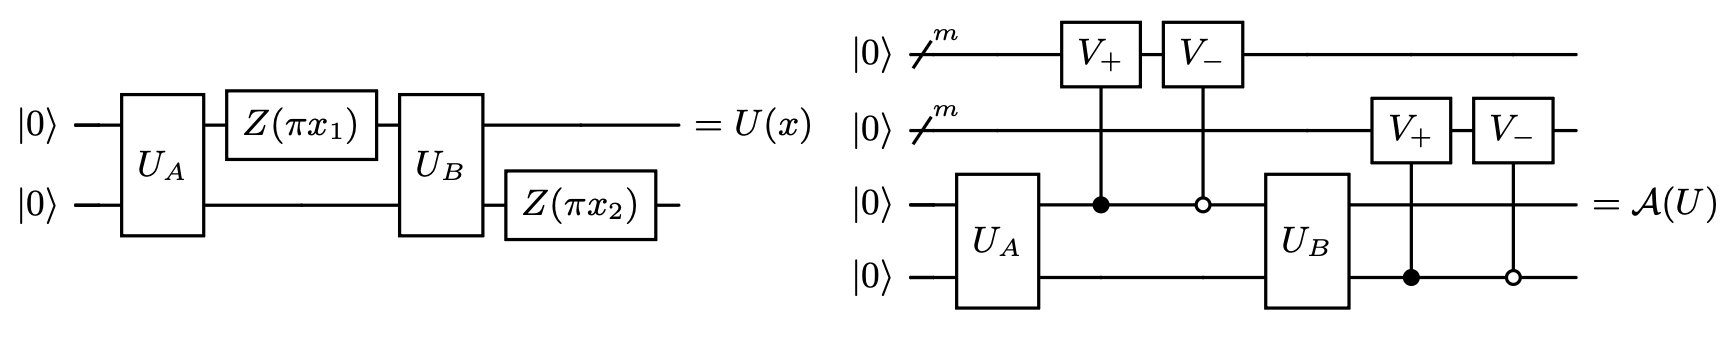
\includegraphics[width=\linewidth]{algorithm_A_circuit.png}\\[-0.3em]
      {\tiny\itshape Left: a 2-qubit Pauli-encoded \(U(\xvec)\).
       Right: the compiled \(A(U)\). The \(V_\pm\) blocks per encoding
       gate stand in for the \(D{\cdot}G{\cdot}D\) construction
       (next slide). \emph{Figure 1 of Barthe \emph{et al.}, 2025.}}
    \end{column}
  \end{columns}

  \note{%
    Two beats to deliver verbally:
    (i) the new circuit \(A(U)\) operates on \(n+1+d\lceil\log L\rceil\)
    qubits and is \emph{not} parametrized -- it is what you would
    compile and ship to a QPU once and re-use across all training
    examples that share the same fixed-gate structure \(\xvec\);
    (ii) the frequency register has \emph{circular} boundary
    conditions, which is what keeps \(V_\pm\) unitary at the edges --
    we will need this for the inductive correctness proof on the next
    slide.
  }
\end{frame}

% =====================================================================
%  SLIDE 10 -- Algorithm A: the D-G-D transformation
% =====================================================================
\begin{frame}{Algorithm \(A\)\,---\,the \(D\!\cdot\!G\!\cdot\!D\) transformation}

  \scriptsize
  \textbf{Setup.}~~WLOG every encoding gate is
  \(V_l(\avec)=\exp\!\bigl(i\pi\alpha_{s_l}P_l\bigr)\) with
  \(P_l=\prod_{k:b_{l,k}=1}Z_k\) (\(X,Y\) are absorbed into the fixed gates).
  Algorithm \(A\) replaces it by
  \(\;\boxed{\;V_l(\avec)\;\longmapsto\;
             D(b_l)\cdot G(s_l)\cdot D(b_l)\;}\)

  \begin{columns}[T,onlytextwidth]
    \begin{column}{0.54\textwidth}
      \scriptsize
      \begin{description}\setlength\itemsep{1pt}
        \item[\(D(b_l)\)]<2-> CNOT cascade
              \(\prod_{k:b_{l,k}=1}\!\mathrm{CNOT}^{(c_k\to a)}\),
              writes parity
              \(\,p_l(k)=\bigoplus_{j:b_{l,j}=1}\!k_j\in\{0,1\}\) onto~\(a\).
        \item[\(G(s_l)\)]<3-> parity-controlled increment / decrement of
              \(f_{s_l}\): apply \(V_+\) when \(p_l=1\), \(V_-\) when
              \(p_l=0\).
        \item[\(D(b_l)\)]<4-> second cascade uncomputes \(a\) to \(\ket{0}\)
              (\(D^{2}=I\)), so the ancilla is reusable.
      \end{description}

      \medskip
      \uncover<5->{\textbf{Net effect.}~The phase
      \(e^{i\pi\alpha_{s_l}\sigma_l(k)}\) of \(V_l(\avec)\) becomes an
      additive shift of \(f_{s_l}\):
      \[
        \ket{l}_f\ket{0}_a\ket{k}_c\!\longmapsto\!
        \ket{l\!+\!e_{s_l}\sigma_l(k)}_f\ket{0}_a\ket{k}_c,\;
        \sigma_l\!=\!(-1)^{1\oplus p_l}.
      \]
      Accumulated over the \(L\) gates this builds \(\vec l\) of Lemma~1
      (correctness proof next slide).}
    \end{column}
    \begin{column}{0.44\textwidth}
      \centering
      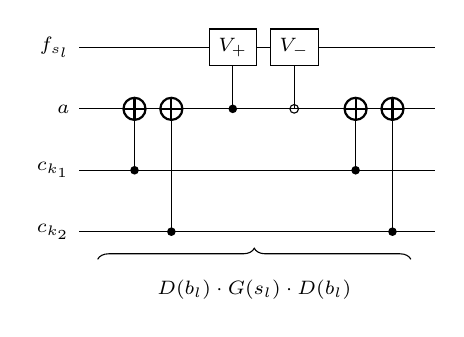
\begin{tikzpicture}[scale=0.78,
          every node/.style={font=\scriptsize},
          targ/.pic={\draw[thick] (0,0) circle (0.14);
                     \draw[thick] (-0.14,0)--(0.14,0);
                     \draw[thick] (0,-0.14)--(0,0.14);}]
        % wires
        \draw (-0.4,3) node[left] {$f_{s_l}$} -- (5.4,3);
        \draw (-0.4,2) node[left] {$a$}       -- (5.4,2);
        \draw (-0.4,1) node[left] {$c_{k_1}$} -- (5.4,1);
        \draw (-0.4,0) node[left] {$c_{k_2}$} -- (5.4,0);
        % first D cascade (CNOTs from c_{k_1}, c_{k_2} onto a)
        \pic at (0.5,2) {targ}; \fill (0.5,1) circle (0.07); \draw (0.5,2)--(0.5,1);
        \pic at (1.1,2) {targ}; \fill (1.1,0) circle (0.07); \draw (1.1,2)--(1.1,0);
        % G block: V_+ on |1>_a, V_- on |0>_a
        \fill (2.1,2) circle (0.07); \draw (2.1,2)--(2.1,3);
        \node[draw,fill=white,minimum width=0.55cm,minimum height=0.42cm] at (2.1,3) {$V_+$};
        \draw (3.1,2) circle (0.07); \draw (3.1,2)--(3.1,3);
        \node[draw,fill=white,minimum width=0.55cm,minimum height=0.42cm] at (3.1,3) {$V_-$};
        % second D cascade
        \pic at (4.1,2) {targ}; \fill (4.1,1) circle (0.07); \draw (4.1,2)--(4.1,1);
        \pic at (4.7,2) {targ}; \fill (4.7,0) circle (0.07); \draw (4.7,2)--(4.7,0);
        % bracket
        \draw[decorate,decoration={brace,amplitude=4pt}] (-0.1,-0.45) -- (5.0,-0.45)
            node[midway,below=4pt,font=\scriptsize]
            {$D(b_l)\cdot G(s_l)\cdot D(b_l)$};
      \end{tikzpicture}
      \\[0.2em]
      {\tiny\itshape One block; two relevant \(c\)-qubits
       (\(b_{l,k_1}\!=\!b_{l,k_2}\!=\!1\)). The two
       \(D\) cascades sandwich \(G\) and reset \(a\).}
    \end{column}
  \end{columns}

  \note{%
    Two key intuitions to deliver verbally:
    (i) \(D\!\cdot\!G\!\cdot\!D\) is the standard ``compute parity --
    do the work -- uncompute'' pattern, just borrowed from reversible
    classical computing; the ancilla is a borrowed scratchpad that ends
    in \(\ket{0}\) so it is reusable across blocks.
    (ii) the \emph{key trick}: the original gate \(V_l(\avec)\)
    multiplies the state by a phase
    \(e^{i\pi\alpha_{s_l}(-1)^{p_l(k)}}\); we replace that
    \(\avec\)-dependent phase by a basis-state shift on a brand-new
    register. The phase will reappear when we eventually multiply by
    \(e^{i\pi\avec\cdot\vec l}\) at read-out time -- but for now we
    have decoupled \(\avec\) entirely from the circuit.
  }
\end{frame}

% =====================================================================
%  SLIDE 11 -- Algorithm A: correctness by induction (Theorem 1)
% =====================================================================
\begin{frame}{Algorithm \(A\)\,---\,correctness by induction (Theorem 1)}

  \begin{block}{\small Theorem 1 (Barthe \emph{et al.}, Sec.~III)}
    \scriptsize
    For every Pauli-encoded \(U\), the parameter-free circuit \(A(U)\)
    prepares
    \(\;\ket{\phi'}=A(U)\ket{0}=
       \sum_{k,\vec l\in[-L,L]^d}\!a_{\vec l,k}\,
       \ket{\vec l}_{f}\ket{0}_{a}\ket{k}_{c}\;\)
    in \(\mathrm{poly}(n,d)\) qubits/gates, with \emph{no knowledge of
    \(\avec\)}. Equivalently, \(A\) physically tags the Fourier indices
    of Lemma~1.
  \end{block}

  \scriptsize
  \uncover<2->{\textbf{Proof.}~Induction on the number of processed gates, with
  invariant
  \(\;\ket{\phi'_t}\!=\!\sum_{k,\vec l}\,a^{(t)}_{\vec l,k}\,
    \ket{\vec l}_f\ket{0}_a\ket{k}_c\),
  where \(a^{(t)}_{\vec l,k}\) are the Lemma~1 amplitudes of the
  truncated circuit \(U_{\le t}\).}

  \vspace{-0.1em}
  \begin{columns}[T,onlytextwidth]
    \begin{column}{0.32\textwidth}
      \scriptsize
      \uncover<3->{\textbf{1.\ Base.} \(A(I)\ket{0}=\ket{0}_f\ket{0}_a\ket{0}_c\) =
      Lemma 1 for \(U=I\). \checkmark}
    \end{column}
    \begin{column}{0.34\textwidth}
      \scriptsize
      \uncover<4->{\textbf{2.\ Fixed gate \(U^{(c)}\).}
      Lifted as \(I^{(f)}\!\otimes\!I^{(a)}\!\otimes\!U^{(c)}\):
      \(\,a^{(t+1)}_{\vec l,k}=\sum_{k'}\!U_{kk'}a^{(t)}_{\vec l,k'}\),
      frequencies untouched. \checkmark}
    \end{column}
    \begin{column}{0.34\textwidth}
      \scriptsize
      \uncover<5->{\textbf{3.\ Encoding gate \(\{s_l,b_l\}\).}
      \(D\!\cdot\!G\!\cdot\!D\) sends
      \(a^{(t)}_{\vec l,k}\!\to\!a^{(t+1)}_{\vec l+e_{s_l}\sigma_l(k),\,k}\),
      matching \(e^{i\pi\alpha_{s_l}P_l}\) on
      \(\sum a^{(t)}\!e^{i\pi\avec\cdot\vec l}\ket k\). \checkmark}
    \end{column}
  \end{columns}

  \vspace{0.2em}
  \begin{alertblock}<6->{\small Why this matters}
    \scriptsize
    \(A\) is \emph{deterministic} and \emph{universal} (across Pauli-encoded
    \(U\)) and amplitude-encodes Lemma 1's spectrum with polynomial
    overhead. Sandwiching \(A\) into a Hadamard test on
    \(\ket{\vec l}_{f}\) yields each \(b_{\vec l}(\xvec)\) up to
    additive error (Corollaries~1 \& 2, next slide).
  \end{alertblock}

  \note{%
    Two intuitions to deliver verbally:
    (i) the inductive invariant is \emph{the same expansion} as
    Lemma~1 -- \(A\) just promotes the formal index \(\vec l\) to a
    physical basis state;
    (ii) the encoding-gate step is the only non-trivial one: the
    matching follows from the calculation of the previous slide
    (continuous phase \(\leftrightarrow\) basis-state shift), modulo
    the parity convention \(\sigma_l(k)=(-1)^{1\oplus p_l(k)}\).
    The full algebraic check (Eqs.~(C9)--(C13) of the paper) is in the
    appendix; the slide gives the \emph{structure} of the argument.
  }
\end{frame}

% =====================================================================
%  SLIDE 12 -- Corollary 1: amplitude-encoded Fourier state
% =====================================================================
\begin{frame}{Amplitude-Encoding the Coefficients\;{\small (Corollary 1)}}

  \footnotesize
  Theorem~1 lifts a circuit to its \emph{state-level} Fourier expansion.
  Sandwiching \(A(U)\) around an observable \(P\) lifts that further to
  the \emph{expectation-value} Fourier expansion -- an amplitude encoding
  of \(\bvec(\xvec)\) on the frequency register.

  \begin{block}{\small Corollary 1 -- Expectation-value Fourier state (Eq.~(9))}
    \scriptsize
    With \(A(U,P)\coloneqq\bigl(\bra{0}_a\bra{0}_c\bigr)\,A(U)^{\dagger}\,P\,A(U)\),
    \[
        A(U,P)\;\ket{0}_f\ket{0}_a\ket{0}_c
        \;=\;
        \frac{1}{\|\bvec(\xvec)\|_2}\!\sum_{\vec l\in\Lspace}\!b_{\vec l}(\xvec)\;
            \ket{\vec l}_f
        \;\;+\;\ket{\dots}_f\,\ket{0_\perp}_{ac}.
    \]
    Post-selection on \(\ket{0}_a\!\ket{0}_c\) succeeds with probability
    \(p_\star=\|\bvec(\xvec)\|_2^{2}\); the surviving \(f\)-register
    amplitude-encodes the Fourier coefficients of
    \(f_{\avec}(\xvec)=\bra{0}U^{\dagger}(\xvec,\avec)\,P\,U(\xvec,\avec)\ket{0}\).
  \end{block}

  \vspace{-0.2em}
  \centering
  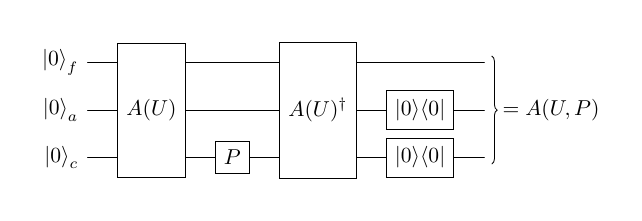
\begin{tikzpicture}[scale=0.78, transform shape]
    \node {\begin{quantikz}[row sep={22pt,between origins}, column sep=14pt, thin lines]
      \lstick{$\ket{0}_f$} & \gate[3]{A(U)} & \qw      & \gate[3]{A(U)^{\dagger}} & \qw                       & \qw \rstick[3]{$=A(U,P)$} \\
      \lstick{$\ket{0}_a$} &                & \qw      &                          & \gate{\ket{0}\!\bra{0}}   & \qw \\
      \lstick{$\ket{0}_c$} &                & \gate{P} &                          & \gate{\ket{0}\!\bra{0}}   & \qw
    \end{quantikz}};
  \end{tikzpicture}\\[-0.1em]
  {\tiny\itshape Compound circuit \(A(U,P)\); projecting
   \(\ket{0}\!\bra{0}\) on \(a,c\) leaves \(\bvec(\xvec)\)
   amplitude-encoded on \(f\). \emph{Redrawn from Fig.~2,
   Barthe \emph{et al.}\ (2025).}}

  \note{%
    Stress this is a \emph{heralded} state-preparation primitive: every
    invocation either succeeds (\(\ket0_a\ket0_c\)) and produces the
    amplitude-encoded Fourier state on \(f\), or fails and is
    discarded. \(p_\star=\|\bvec(\xvec)\|_2^{2}\) is bounded below for
    the concept classes the paper considers. Next slide turns this
    state into a \emph{measurement} protocol via a Hadamard test.
  }
\end{frame}

% =====================================================================
%  SLIDE 13 -- Corollary 2: Hadamard test extraction
% =====================================================================
\begin{frame}{Hadamard-Test Coefficient Estimation\;{\small (Corollary 2)}}

  \footnotesize
  Corollary~1 amplitude-encodes \(\bvec(\xvec)\) on the \(f\)-register;
  Corollary~2 turns that into a single-number estimate of any chosen
  \(b_{\vec l}\) via a controlled-\(A(U,P)\) Hadamard test.

  \begin{block}{\small Corollary 2 -- Hadamard-test extraction (Sec.~III)}
    \scriptsize
    For every \(\vec l\in\Lspace\) there exist two
    \(\mathrm{poly}(n,d)\)-depth circuits returning
    \(\Re b_{\vec l}(\xvec)\) and \(\Im b_{\vec l}(\xvec)\) as the
    bias of a binary measurement on the ancilla; after
    \(N=O\bigl(\varepsilon_b^{-2}\log\delta^{-1}\bigr)\) shots,
    \[
        \Pr\!\bigl[\;|\hat b_{\vec l}(\xvec)-b_{\vec l}(\xvec)|\le\varepsilon_b\;\bigr]
        \;\ge\;1-\delta.
    \]
    Total cost over all \(|\Lspace|=m\) frequencies:
    \(O(m\,\varepsilon_b^{-2}\log\delta^{-1})\) circuit executions.
  \end{block}

  \vspace{-0.2em}
  \centering
  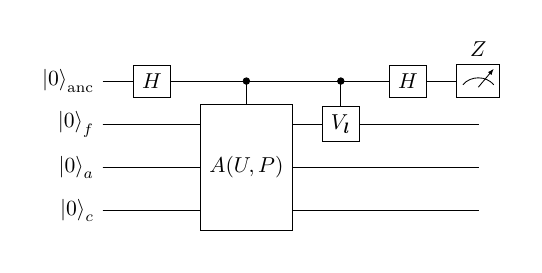
\begin{tikzpicture}[scale=0.78, transform shape]
    \node {\begin{quantikz}[row sep={20pt,between origins}, column sep=14pt, thin lines]
      \lstick{$\ket{0}_{\mathrm{anc}}$} & \gate{H}  & \ctrl{1}            & \ctrl{1}             & \gate{H}  & \meter{Z} \\
      \lstick{$\ket{0}_f$}              & \qw       & \gate[3]{A(U,P)}    & \gate{V_{\vec l}}    & \qw       & \qw \\
      \lstick{$\ket{0}_a$}              & \qw       &                     & \qw                  & \qw       & \qw \\
      \lstick{$\ket{0}_c$}              & \qw       &                     & \qw                  & \qw       & \qw
    \end{quantikz}};
  \end{tikzpicture}\\[-0.1em]
  {\tiny\itshape Hadamard test for \(\Re b_{\vec l}\): the final
   \(H\!\cdot\!Z\) gives \(\Pr[0]-\Pr[1]=\Re b_{\vec l}\) (insert
   \(S^{\dagger}\) before the last \(H\) for \(\Im b_{\vec l}\)).
   \emph{Redrawn from Fig.~3, Barthe \emph{et al.}\ (2025).}}

  \note{%
    Walk through the protocol: controlled-\(A(U,P)\) puts the Fourier
    state on the data registers conditioned on the ancilla; the
    controlled-\(V_{\vec l}\) (an integer-shift selector indexed by
    \(\vec l\)) interferes the \(\vec l\)-component with the rest;
    the final Hadamard reads the bias.
    \(\Pr[0]-\Pr[1]=\Re b_{\vec l}\) (insert \(S^{\dagger}\) before
    the final \(H\) for \(\Im b_{\vec l}\)).
    \(\varepsilon_b^{-2}\) shots follow from Hoeffding.
    Sec.~III thus collapses to one quantum primitive
    \(\texttt{extract\_b}(\xvec,\vec l)\to\hat b_{\vec l}\); the rest
    of the learner is classical (LASSO, generalisation, Hamiltonian
    transfer).
  }
\end{frame}

% =====================================================================
%  SLIDE 14 -- Classical stage: LASSO regression
% =====================================================================
\begin{frame}{Classical Stage: LASSO Regression on \(\hat{\bvec}(\xvec)\)}

  \footnotesize
  Algorithm \(A\) hands the regressor a noisy feature matrix
  \(\hat B\) and noisy labels \(\hat{\vec y}\); learning collapses to a
  constrained linear regression in the (parameter-free) features
  \(\bvec(\xvec)\).

  \begin{block}{\small Noise model (Eqs.~A1--A3 of Barthe \emph{et al.})}
    \scriptsize
    \[
      \underbrace{b_{\vec l}(\xvec_t)\!\cdot\!w_{\vec l}(\avec)=y_t}_{\text{linear truth}},
      \quad
      \underbrace{\hat{\bvec}(\xvec_t)=\bvec(\xvec_t)+\vec\eta_{b,t},\;
       \|\vec\eta_{b,t}\|_\infty\!\le\!\varepsilon_b}_{\text{Hadamard-test noise (Cor.~2)}},
      \quad
      \underbrace{\hat y_t=y_t+\eta_{y,t},\;|\eta_{y,t}|\!\le\!\varepsilon_y}_{\text{label noise}}.
    \]
  \end{block}

  \begin{block}<2->{\small LASSO objective\;\(\bigl[\,\Hyp=\{\bvec\!\mapsto\!\bvec\!\cdot\!\wvec\,:\,\|\wvec\|_1\le\Lambda_1\}\,\bigr]\)}
    \scriptsize
    \[
        \hat{\wvec}\;=\;\arg\min_{\|\wvec\|_1\le\Lambda_1}
            \bigl\|\,\hat{\vec y}-\hat B\,\wvec\,\bigr\|_2^{2},
        \qquad
        \hat B_{t,\vec l}\!=\!\hat b_{\vec l}(\xvec_t),\quad
        \Lambda_1\!\ge\!\|\wvec(\avec)\|_1.
    \]
    \emph{Inductive bias.}~\(\wvec(\avec)\) lies on the torus
    \(\{e^{i\pi\vec l\cdot\avec}\}\) so \(\|\wvec\|_\infty\!=\!1\) and
    \(\Lambda_1\) need only scale with \(m=|\Lspace|\), not \(2^{m}\).
  \end{block}

  \footnotesize
  \uncover<3->{\(\Rightarrow\) the \emph{generalisation guarantee} that
  \(\hat{\wvec}\) is close to \(\wvec(\avec)\) on
  \(\Dist\)-distributed test points is Theorem~6 -- next slide.}

  \note{%
    Two beats to deliver:
    (i) feature-noise from Cor.~2 is \emph{\(\ell_\infty\)-bounded}, not
    Gaussian -- this matters because the LASSO bound (Theorem 6) is
    proven against worst-case adversarial perturbations of bounded
    \(\ell_\infty\) magnitude, so it transfers verbatim;
    (ii) the inductive bias \(\|\wvec\|_\infty\!=\!1\) on the torus is
    what saves us from paying for the exponentially-large feature
    dimension at test time -- LASSO's sample-complexity scales with
    \(\Lambda_1\), not \(m\) directly.
  }
\end{frame}

% =====================================================================
%  SLIDE 15 -- Theorem 6 generalisation bound
% =====================================================================
\begin{frame}{Generalisation Guarantee\;{\small (Theorem 6)}}

  \footnotesize
  Theorem~6 controls the \emph{true} mean-square risk
  \(L_c(h)=\mathbb E_{\xvec\sim\Dist}[(h(\xvec)-c_{\avec}(\xvec))^{2}]\)
  of the LASSO minimiser \(\hat h(\xvec)=\hat{\wvec}\!\cdot\!\hat{\bvec}(\xvec)\)
  in terms of (i) the sample size \(T\), (ii) the feature noise
  \(\varepsilon_b\), and (iii) the label noise \(\varepsilon_y\).

  \begin{block}{\small Theorem 6 -- LASSO under \(\ell_\infty\)-bounded perturbations}
    \scriptsize
    Let \(r_\infty\!\coloneqq\!\sup_{\xvec}\|\bvec(\xvec)\|_\infty\).
    If
    \[
        T\;\ge\;\frac{(2\Lambda_1\,r_\infty)^{4}\sqrt{2\log(2m/\delta)}}{\varepsilon^{2}},
        \qquad
        \Lambda_1\,\varepsilon_b\;\le\;0.2\,\varepsilon,
        \qquad
        \varepsilon_y\;\le\;0.5\,\varepsilon,
    \]
    then with probability at least \(1-\delta\),
    \(\;L_c(\hat h)\le\varepsilon\).
  \end{block}

  \vspace{-0.2em}
  \begin{columns}[T,onlytextwidth]
    \begin{column}{0.50\textwidth}
      \scriptsize
      \uncover<2->{\textbf{Resource trade-off.}
      \begin{itemize}\setlength\itemsep{1pt}
        \item Sample budget: \(T\!=\!\tilde\Theta\bigl((\Lambda_1 r_\infty)^{4}/\varepsilon^{2}\bigr)\)
              -- \emph{poly} in the feature dimension \(m\) only via
              \(\Lambda_1\).
        \item Quantum budget: \(\varepsilon_b\!\le\!0.2\varepsilon/\Lambda_1\)
              \(\Rightarrow\) Hadamard-test
              \(N=O(\varepsilon_b^{-2})\) shots per coefficient.
        \item Label budget: \(\varepsilon_y\!\le\!0.5\varepsilon\)
              -- absorbs Trotter / shot noise on the labels.
      \end{itemize}}
    \end{column}
    \begin{column}{0.46\textwidth}
      \scriptsize
      \uncover<3->{\textbf{Specialisation to \(\Cclass^{\PQC}_{\log}\).}\\[-0.2em]
      For the homogeneous PQC class with \(L\) re-uploads,
      \(\Lambda_1=m,\;r_\infty=1\), and Theorem~6 closes to
      \[
          T=\tilde\Theta\!\bigl(m^{4}/\varepsilon^{2}\bigr),
          \quad
          \varepsilon_b=0.2\varepsilon/m
      \]
      -- the closed form Eq.~(14) used in the proof of Theorem~2.}
    \end{column}
  \end{columns}

  \note{%
    Three numbers to drive home verbally:
    (i) sample complexity scales with \((\Lambda_1 r_\infty)^4\), not
    \(2^m\) -- the inductive bias is doing work;
    (ii) the quantum-side knob is \(\varepsilon_b\le0.2\varepsilon/\Lambda_1\),
    which sets the per-coefficient shot budget;
    (iii) Theorem~6 absorbs an independent label noise
    \(\varepsilon_y\le0.5\varepsilon\), which we will need on the
    Hamiltonian-side slides (Trotter error becomes label noise).
  }
\end{frame}

\end{document}